\documentclass[a4paper,12pt]{article}
%%%%%%%%%%%%%%%%%%%%%%%%%%%%%%%%%%%%%%%%%%%%%%%%%%%%%%%%%%%%%%%%%%%%%%%%%%%%%%%%%%%%%%%%%%%%%%%%%%%%%%%%%%%%%%%%%%%%%%%%%%%%%%%%%%%%%%%%%%%%%%%%%%%%%%%%%%%%%%%%%%%%%%%%%%%%%%%%%%%%%%%%%%%%%%%%%%%%%%%%%%%%%%%%%%%%%%%%%%%%%%%%%%%%%%%%%%%%%%%%%%%%%%%%%%%%
\usepackage{eurosym}
\usepackage{vmargin}
\usepackage{amsmath}
\usepackage{graphics}
\usepackage{epsfig}
\usepackage{enumerate}
\usepackage{multicol}
\usepackage{subfigure}
\usepackage{fancyhdr}
\usepackage{listings}
\usepackage{framed}
\usepackage{graphicx}
\usepackage{amsmath}
\usepackage{chngpage}
%\usepackage{bigints}

\usepackage{vmargin}
% left top textwidth textheight headheight
% headsep footheight footskip
\setmargins{2.0cm}{2.5cm}{16 cm}{22cm}{0.5cm}{0cm}{1cm}{1cm}
\renewcommand{\baselinestretch}{1.3}

\setcounter{MaxMatrixCols}{10}

\begin{document}
\large 
\noindent ABC Tech, a Speedboat manufacturing company, was established a few decades back. The
company has shown a consistent growth in its revenue from Speedboat sales since its inception.\\

\noindent However, over the years the company has struggled to keep it’s inventory and production cost
down because of variability in sales and Speedboat demand. The management at ABC Tech is
under enormous pressure from the shareholders and board to reduce the production cost.
Additionally, they are also interested in understanding the impact of their marketing and
customer connect efforts towards overall sales. In the same effort, they have your employer as
a data science and predictive analytics consultant.\\
\medskip

\noindent Your senior have analysed the sales data and believe that ARIMA model will fit the data. They have  suggested you to develop an ARIMA model to forecast sale / demand for next three years.\\
\medskip

\noindent
Additionally, They have  also suggested you to investigate the impact of marketing program on
sales by using an exogenous variable ARIMA model. You agreed on the steps to be followed
and agree on the following steps.\\

\noindent \textit{Note: You will require “Forecast” package for this assignment.}

\newpage 
\noindent Data provided in \texttt{Speedboat\_Sales.csv} in the local file directory.
%%%%%%%%%%%%%%%%%%%%%%%%%%%%%%%%%%%%%%%%%%%%%%%%%%%%%%%%%%%%%%%%%%%%%%%%%%%%%%%%%%%%%%%%%%%%%%


\begin{framed}
\begin{verbatim}
getwd()

data <- read.csv("Speedboat_Sales.csv")

list.files()

head(data)

install.packages("Forecast")
library(Forecast)

\end{verbatim}
\end{framed}


\newpage 

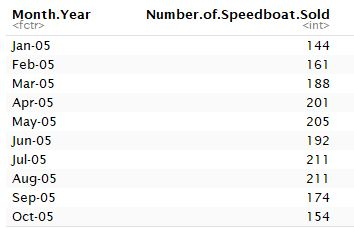
\includegraphics[scale=1.1]{00-B2/images/Speedboat_data.JPG}


%% PART 1
\newpage 

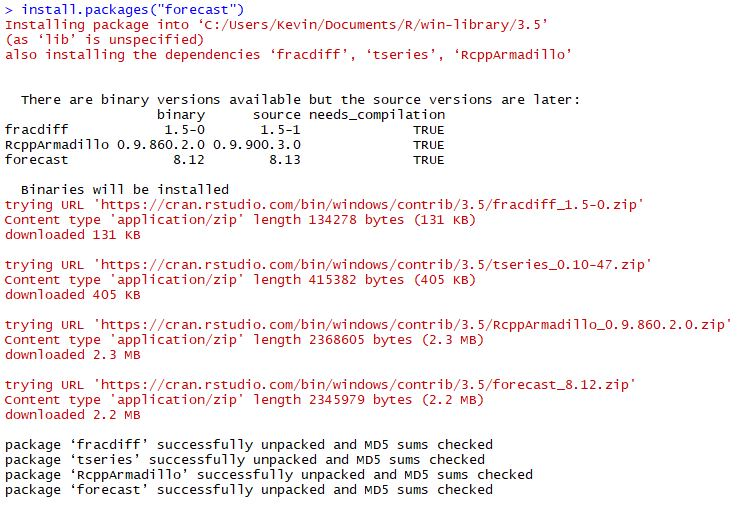
\includegraphics[]{00-B2/images/install_forecast.JPG}

\newpage

\subsection*{Exercise 1}
Plot a time series chart
with year as $X$ axis and sales as $Y$
axis with suitable labelling. Basis the plot thus obtain,
comment on the type of time series.

\begin{framed}
\begin{verbatim}
data = ts(data[,2],start = c(2005,1),frequency = 12)

plot(data, xlab="Years", ylab = "Speedboat Sales")
\end{verbatim}
\end{framed}

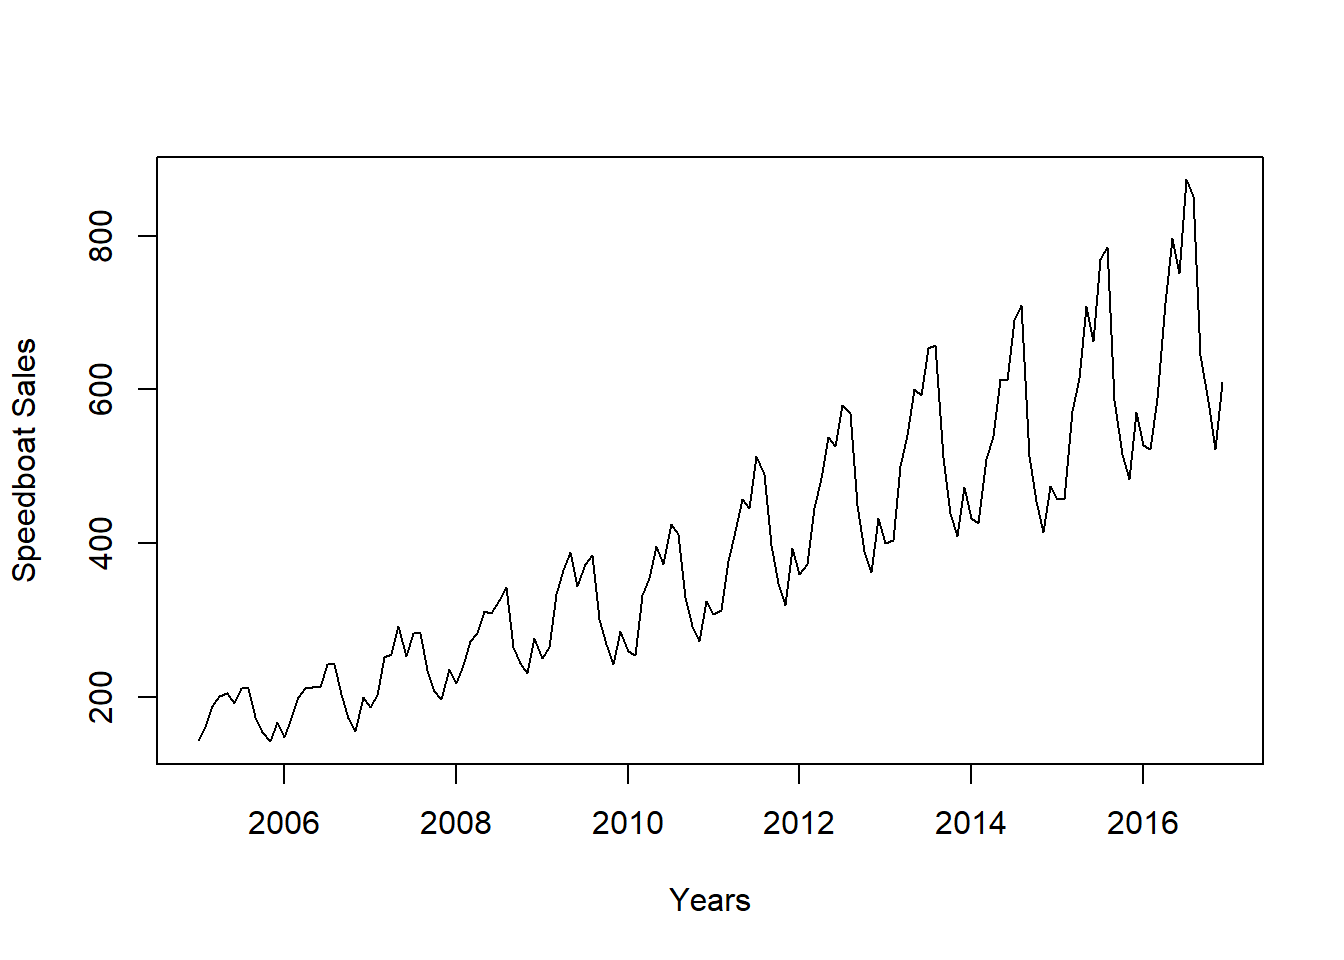
\includegraphics[]{00-B2/images/Speedboat_1.png}
\newpage 
\noindent Clearly the above chart has an upward trend for speedboat sales and there is also a seasonal
component.

%%%%%%%%%%%%%%%%%%%%%%%%%%%%%%%%%%%%%%%%%%%%%%%%%%%%%%%%%%%%%%%%%%%%%%%%%%%%%%%%%%%%%%%%%%%%%%
%% PART 2
\newpage 

\subsection*{Exercise 2}
\noindent Plot ACF and PACF to identify potential AR and MA model for this series and
comment on the results.
\begin{framed}
\begin{verbatim}
par(mfrow = c(1,2))

acf(ts(data),main="ACF Speedboat Sales")
pacf(ts(data),main="PACF Speedboat Sales")
\end{verbatim}
\end{framed}

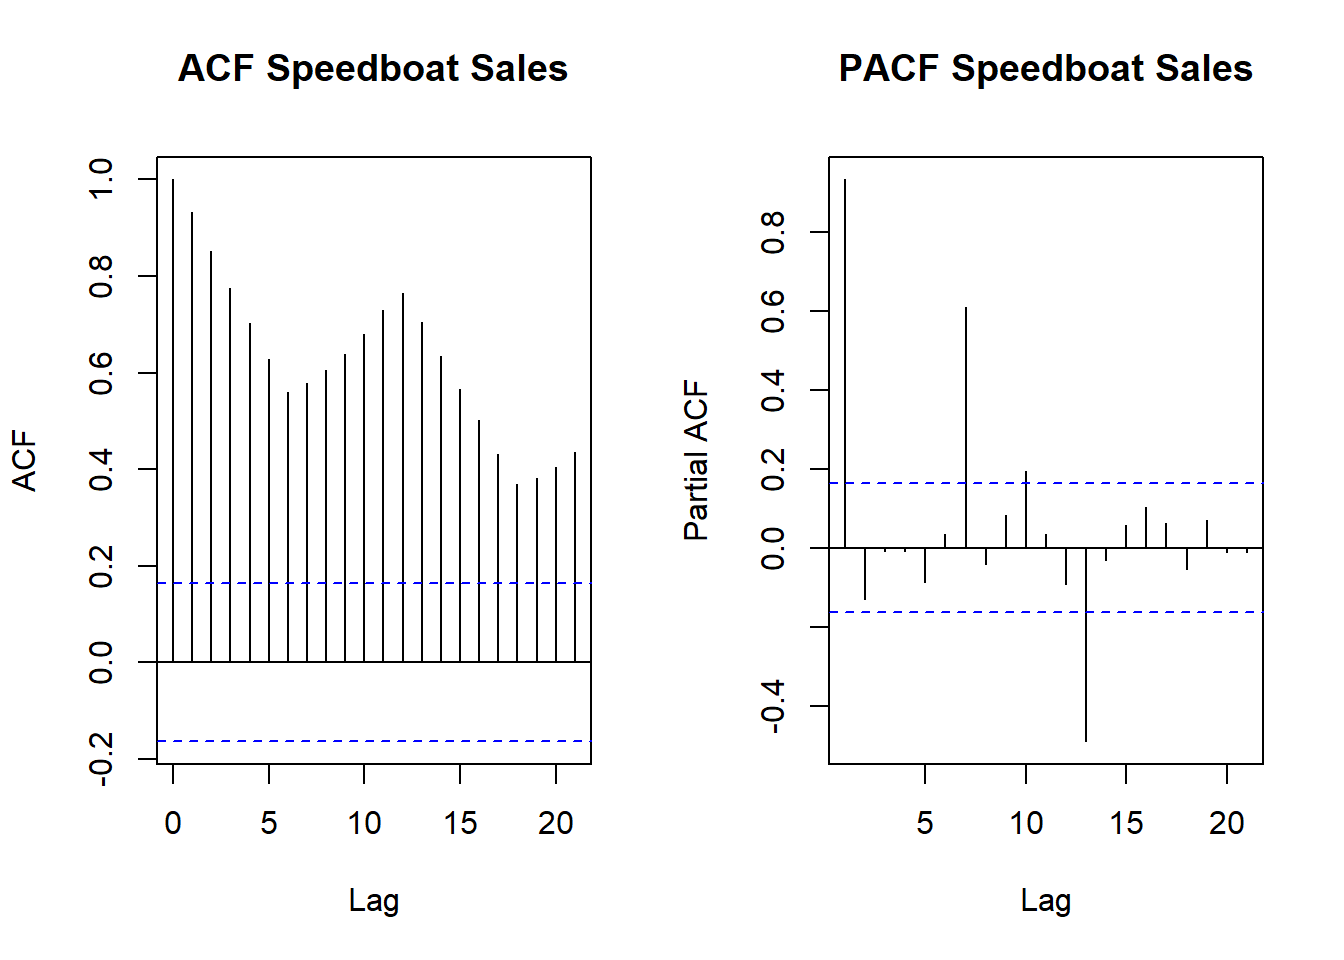
\includegraphics[]{00-B2/images/Speedboat_2.png}


%%%%%%%%%%%%%%%%%%%%%%%%%%%%%%%%%%%%%%%%%%%%%%%%%%%%%%%%%%%%%%%%%%%%%%%%%%%%%%%%%%%%%%%%%%%%%%
%% PART 3
\newpage 

\subsection*{Exercise 3}

\noindent You believe that differencing series is one of the ways to remove trend. Obtain the first
order and second order difference series and plot the same. Also provide comment on
variance of the $d(1)$ series.

\begin{framed}
\begin{verbatim}
par(mfrow = c(1,1))

diff_data = diff(data)
plot(diff_data,ylab="Differenced Speedboat Sales")
\end{verbatim}
\end{framed}
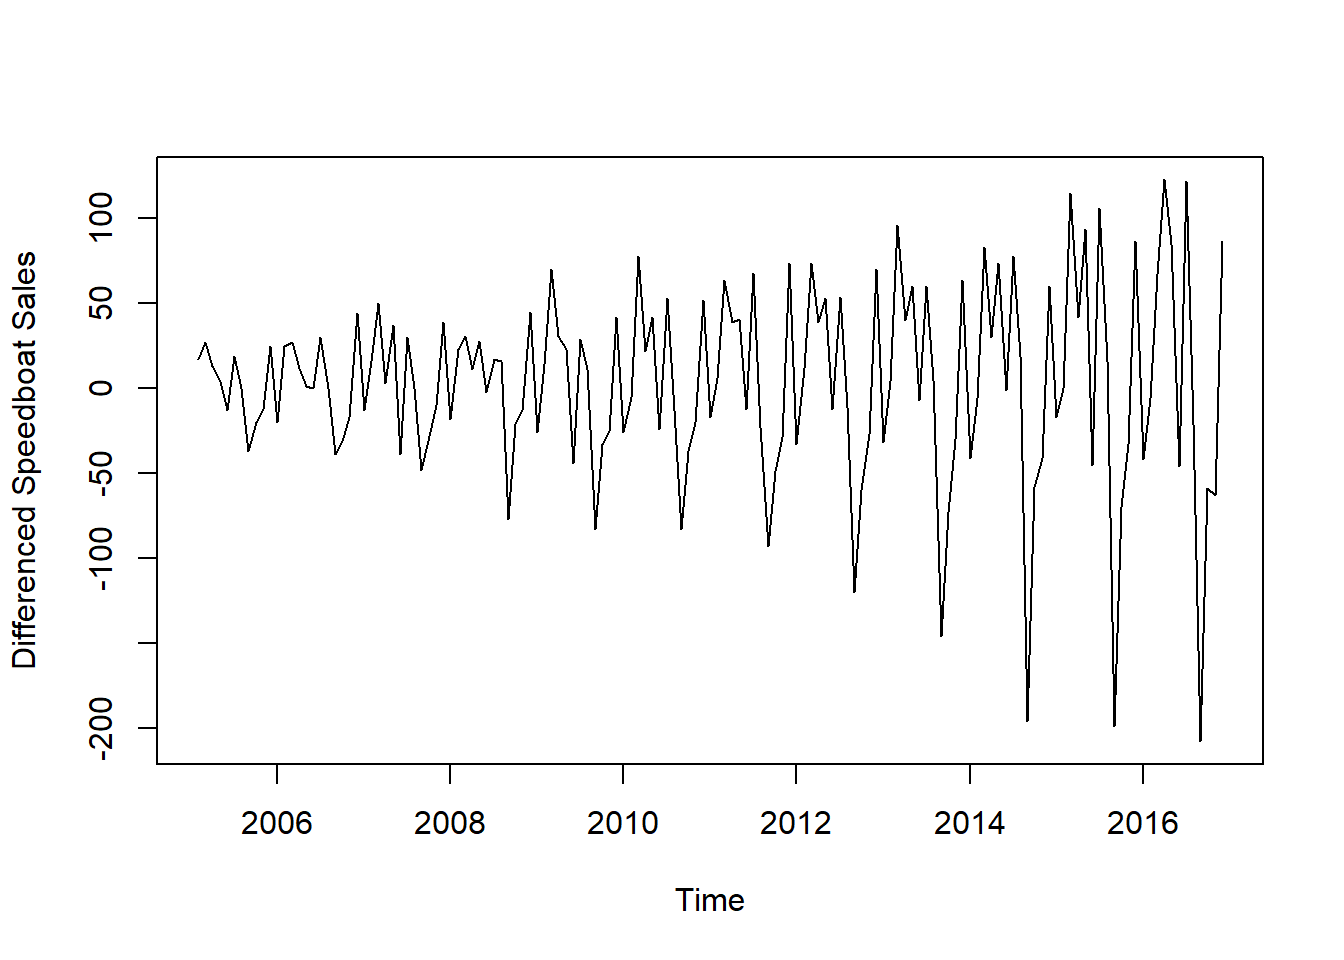
\includegraphics[]{00-B2/images/Speedboat_3.png}
\newpage
\begin{itemize}
    \item The above series ($d=1$) is not stationary on variance i.e. variation in the plot is increasing as we move towards the right of the chart. 
\item We need to make the series stationary on variance to produce reliable
forecasts through ARIMA models.
\end{itemize}

\newpage 

\begin{framed}
\begin{verbatim}
diff_data_2 = diff(diff_data)
plot(diff_data_2,ylab="Differenced Speedboat Sales")
\end{verbatim}
\end{framed}
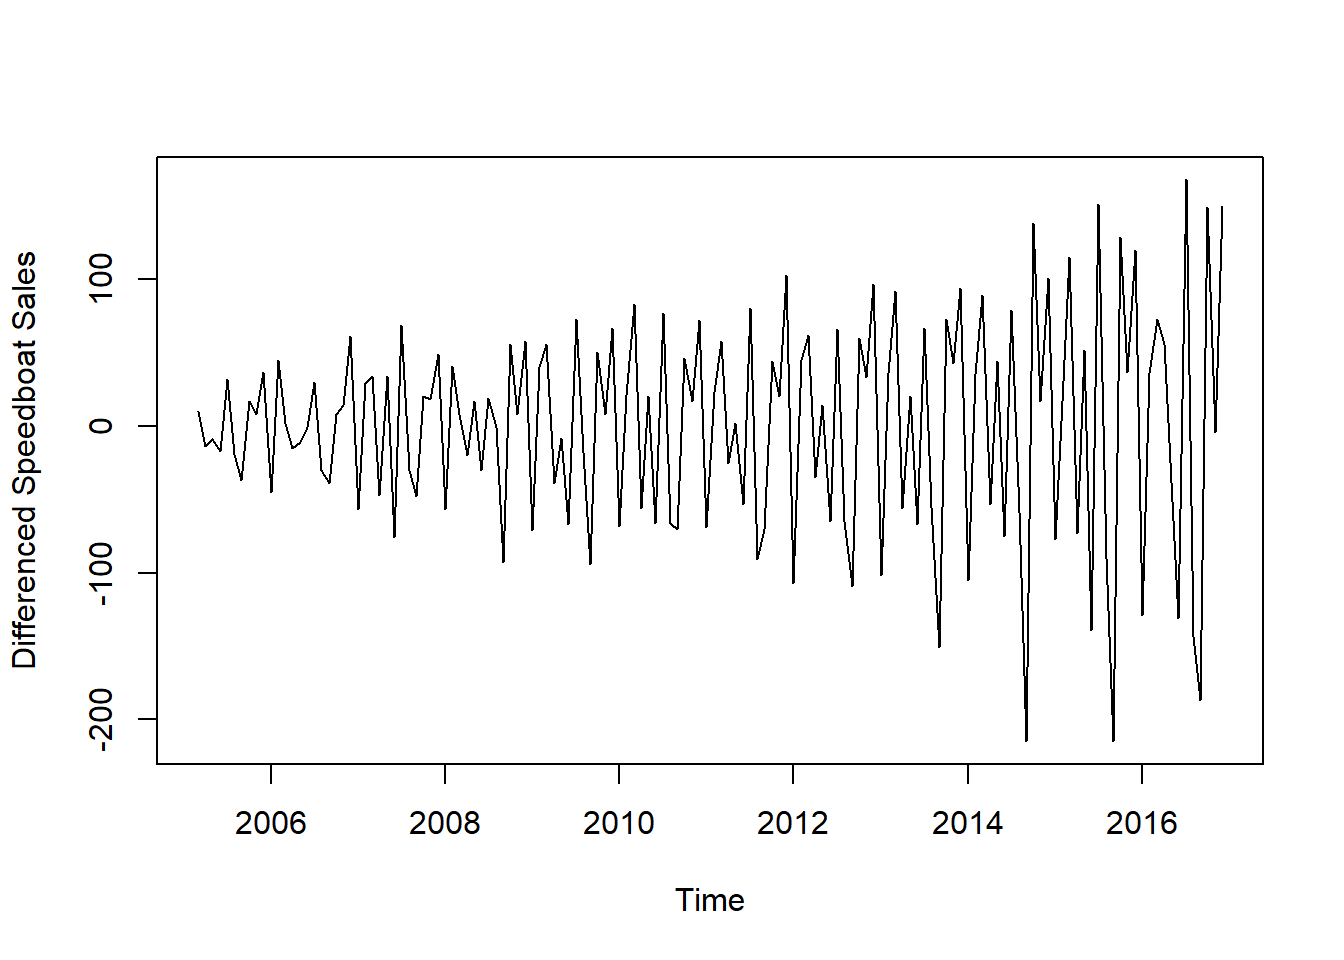
\includegraphics[]{00-B2/images/Speedboat_4.png}






%%%%%%%%%%%%%%%%%%%%%%%%%%%%%%%%%%%%%%%%%%%%%%%%%%%%%%%%%%%%%%%%%%%%%%%%%%%%%%%%%%%%%%%%%%%%%%
%% PART 4

\newpage 

\subsection*{Exercise 4}
\noindent Looking at the plots of difference series, you decide to apply log transformation to the
original series to smoothen the variance. Obtain the log-transformed (base 10) series
and plot the same. 
\begin{framed}
\begin{verbatim}
Log_data = log10(data)

plot(Log_data,ylab="Log Speedboat Sales")
\end{verbatim}
\end{framed}
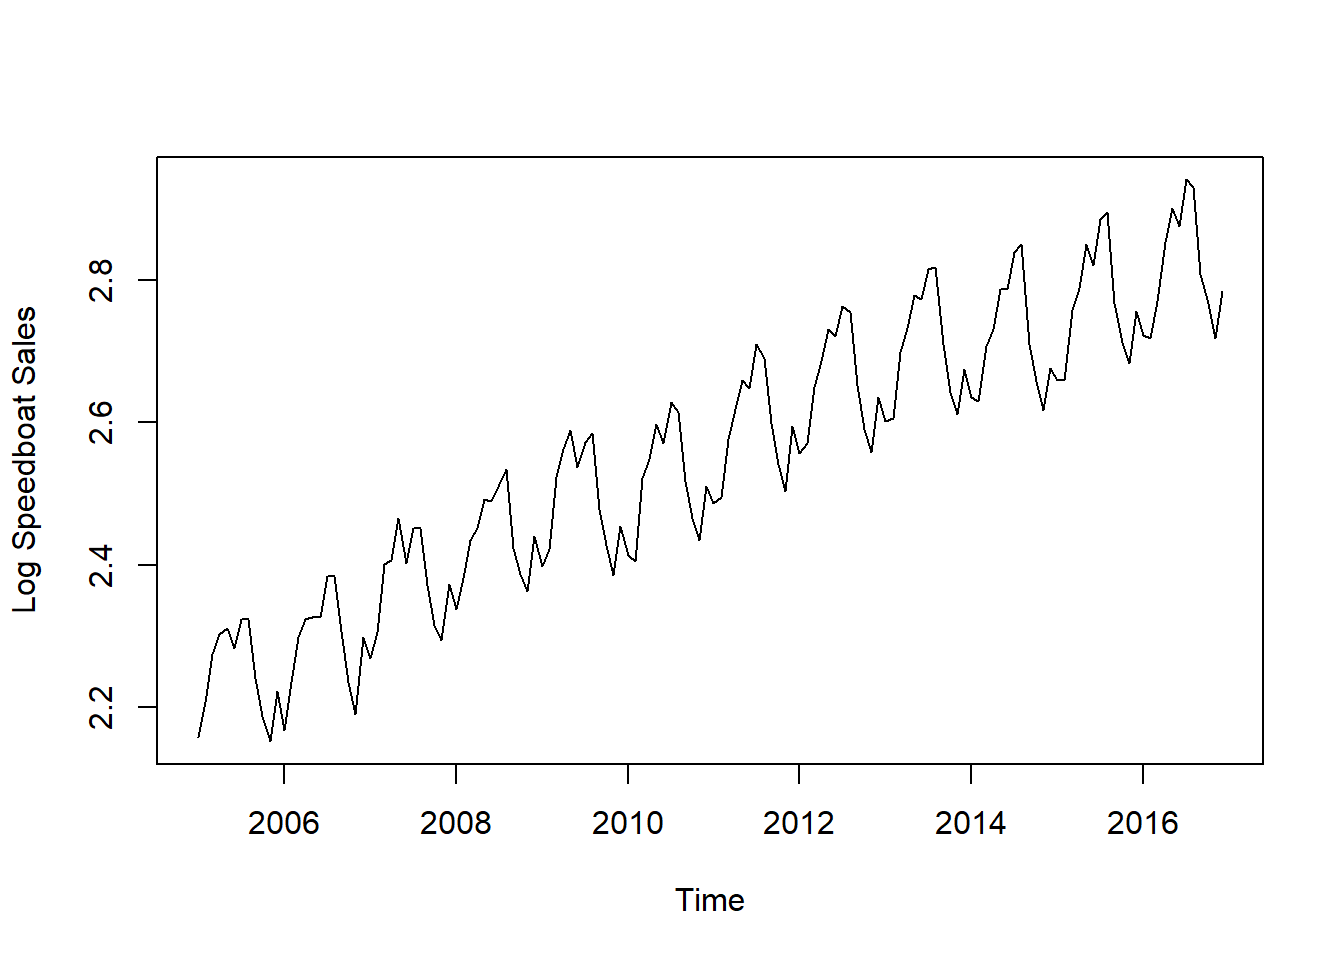
\includegraphics[]{00-B2/images/Speedboat_5.png}


%%%%%%%%%%%%%%%%%%%%%%%%%%%%%%%%%%%%%%%%%%%%%%%%%%%%%%%%%%%%%%%%%%%%%%%%%%%%%%%%%%%%%%%%%%%%%%
%% PART 5
\newpage 

\subsection*{Exercise 5}
\noindent  Obtain the first order difference series of the transformed series and plot the same. 

\begin{framed}
\begin{verbatim}
Diff_log_data = diff(Log_data)

plot(Diff_log_data,ylab="Difference Log Speedboat Sales")
\end{verbatim}
\end{framed}

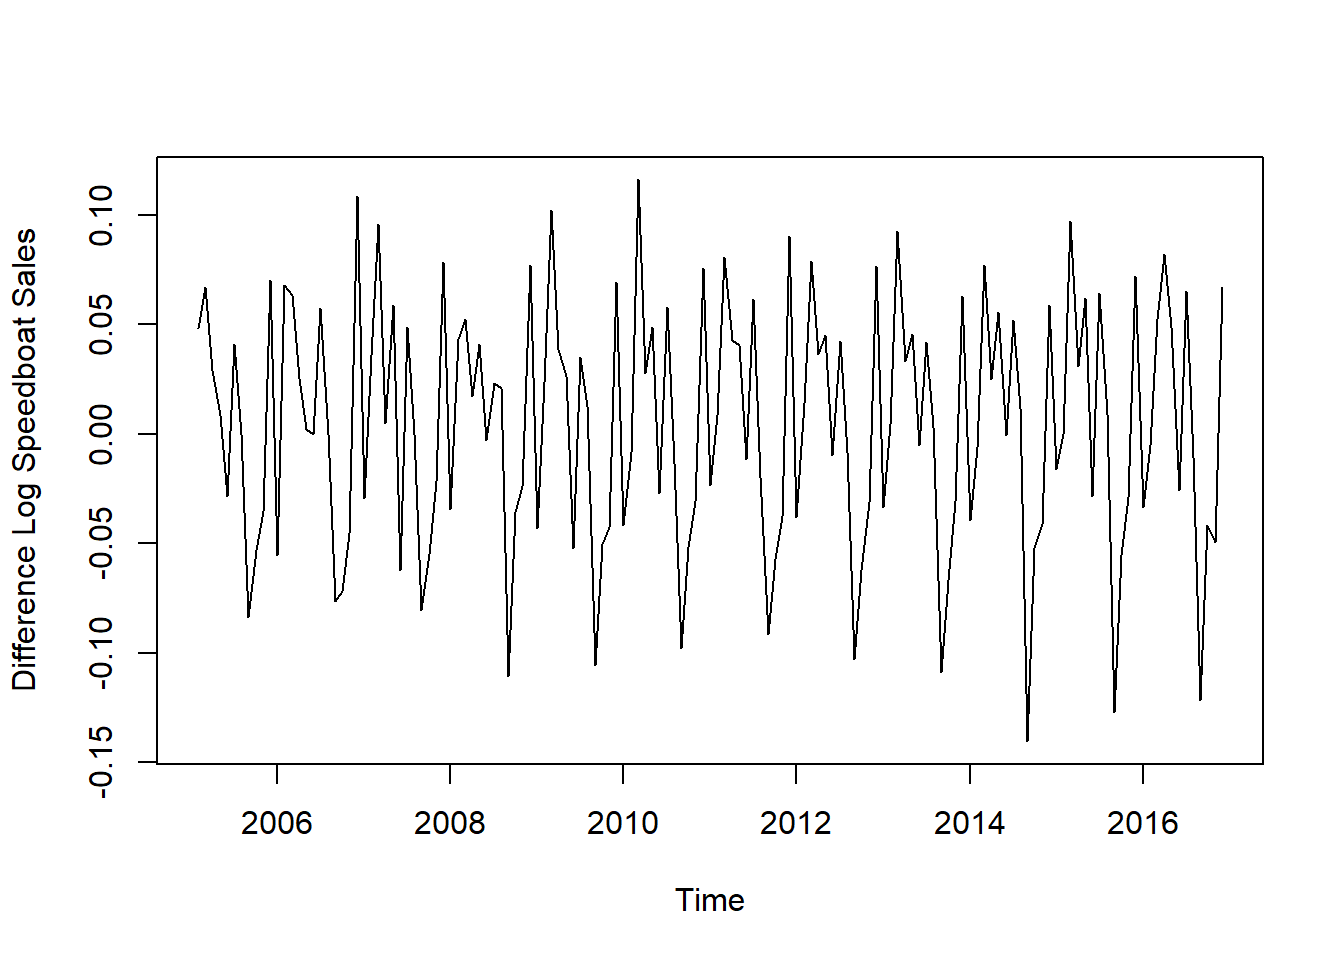
\includegraphics[]{00-B2/images/Speedboat_6.png}

%%%%%%%%%%%%%%%%%%%%%%%%%%%%%%%%%%%%%%%%%%%%%%%%%%%%%%%%%%%%%%%%%%%%%%%%%%%%%%%%%%%%%%%%%%%%%%
%% PART 6
\newpage


\subsection*{Exercise 6}
\noindent Plot ACF and PACF to identify potential AR and MA model for this series and
comment on the results. 

\begin{framed}
\begin{verbatim}
par(mfrow = c(1,2))

acf(ts(Diff_log_data),main="ACF Speedboat Sales")
pacf(ts(Diff_log_data),main="PACF Speedboat Sales")
\end{verbatim}
\end{framed}

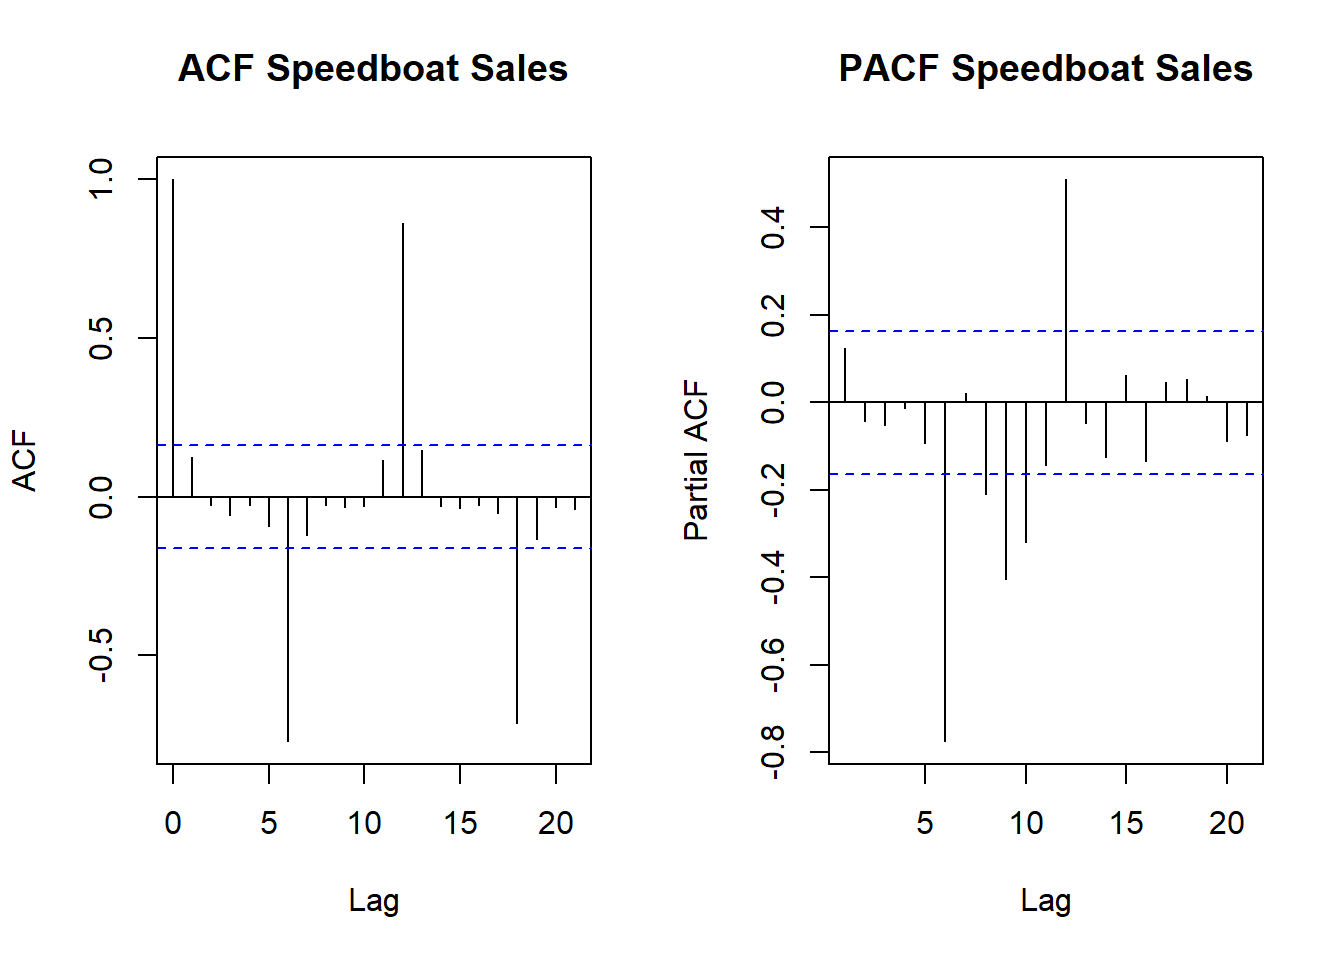
\includegraphics[]{00-B2/images/Speedboat_7.png}

\begin{itemize}
\item Since, there are enough spikes in the plots outside the insignificant zone (dotted horizontal lines) we
can conclude that the residuals are not random. 
\item This implies that there is juice or information available
in residuals to be extracted by AR and MA models.
\item Also, there is a seasonal component available in
the residuals at the lag 12 (represented by spikes at lag 12).
\item This makes sense since we are analyzing
monthly data that tends to have seasonality of 12 months because of patterns in tractor sales.
\end{itemize}

%%%%%%%%%%%%%%%%%%%%%%%%%%%%%%%%%%%%%%%%%%%%%%%%%%%%%%%%%%%%%%%%%%%%%%%%%%%%%%%%%%%%%%%%%%%%%%
%% PART 7
\newpage 

\subsection*{Exercise 7}
\noindent Use Auto arima function in forecast package in R helps us identify the best fit ARIMA
model on the fly. Comment on the summary results of fitting this series and on Akaike
Information Criterion (AIC) and Bayesian Information Criterion (BIC) values. 


\begin{framed}
\begin{verbatim}
ARIMAfit = auto.arima(Log_data,approximation=FALSE,
    trace=FALSE)

summary(ARIMAfit)
\end{verbatim}
\end{framed}

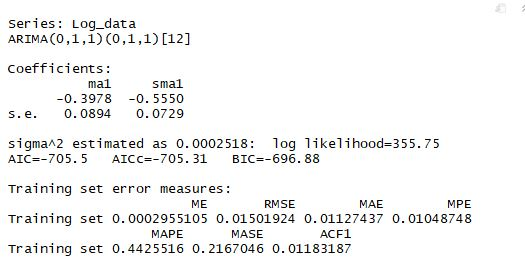
\includegraphics[scale=1.05]{00-B2/images/ModelSummary.JPG}

\newpage 
\begin{itemize}
    \item The best fit model is selected based on Akaike Information Criterion (AIC), and Bayesian Information
Criterion (BIC) values. 
    \item The idea model to choose who has minimum AIC and BIC values.
As expected, our model has I (or integrated) component equal to 1. 
    \item This represents differencing of
order 1. There is additional differencing of lag 12 in the above best fit model. 
    \item  Moreover, the best fit
model has MA value of order 1. Also, there is seasonal MA with lag 12 of order 1.
\end{itemize}


%%%%%%%%%%%%%%%%%%%%%%%%%%%%%%%%%%%%%%%%%%%%%%%%%%%%%%%%%%%%%%%%%%%%%%%%%%%%%%%%%%%%%%%%%%%%%%
%% PART 8
\newpage 


\subsection*{Exercise 8}
Predict speedboat sales for next 3 years i.e. for 2015, 2016, and 2017 through the above
model and plot the results along-with one times the range of standard error from
predicted value. 



\begin{framed}
\begin{verbatim}
par(mfrow = c(1,1))
pred = predict(ARIMAfit, n.ahead = 36)
pred
\end{verbatim}
\end{framed}

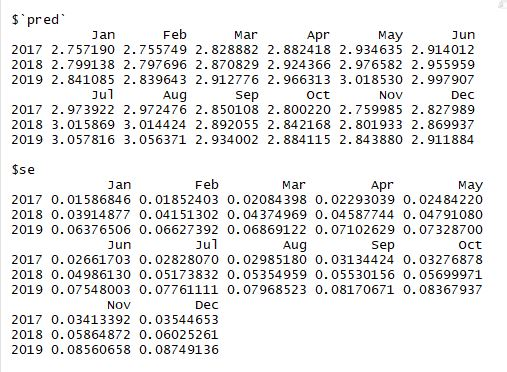
\includegraphics[]{00-B2/images/Preds_SE.JPG}
\newpage 
\begin{framed}
\begin{verbatim}
plot(data,type="l",xlim=c(2006,2020),ylim=c(1,1600),xlab = "Year",ylab = "Speedboat Sales")
lines(10^(pred$pred),col="blue")
lines(10^(pred$pred+2*pred$se),col="orange")
lines(10^(pred$pred-2*pred$se),col="Brown")

\end{verbatim}
\end{framed}
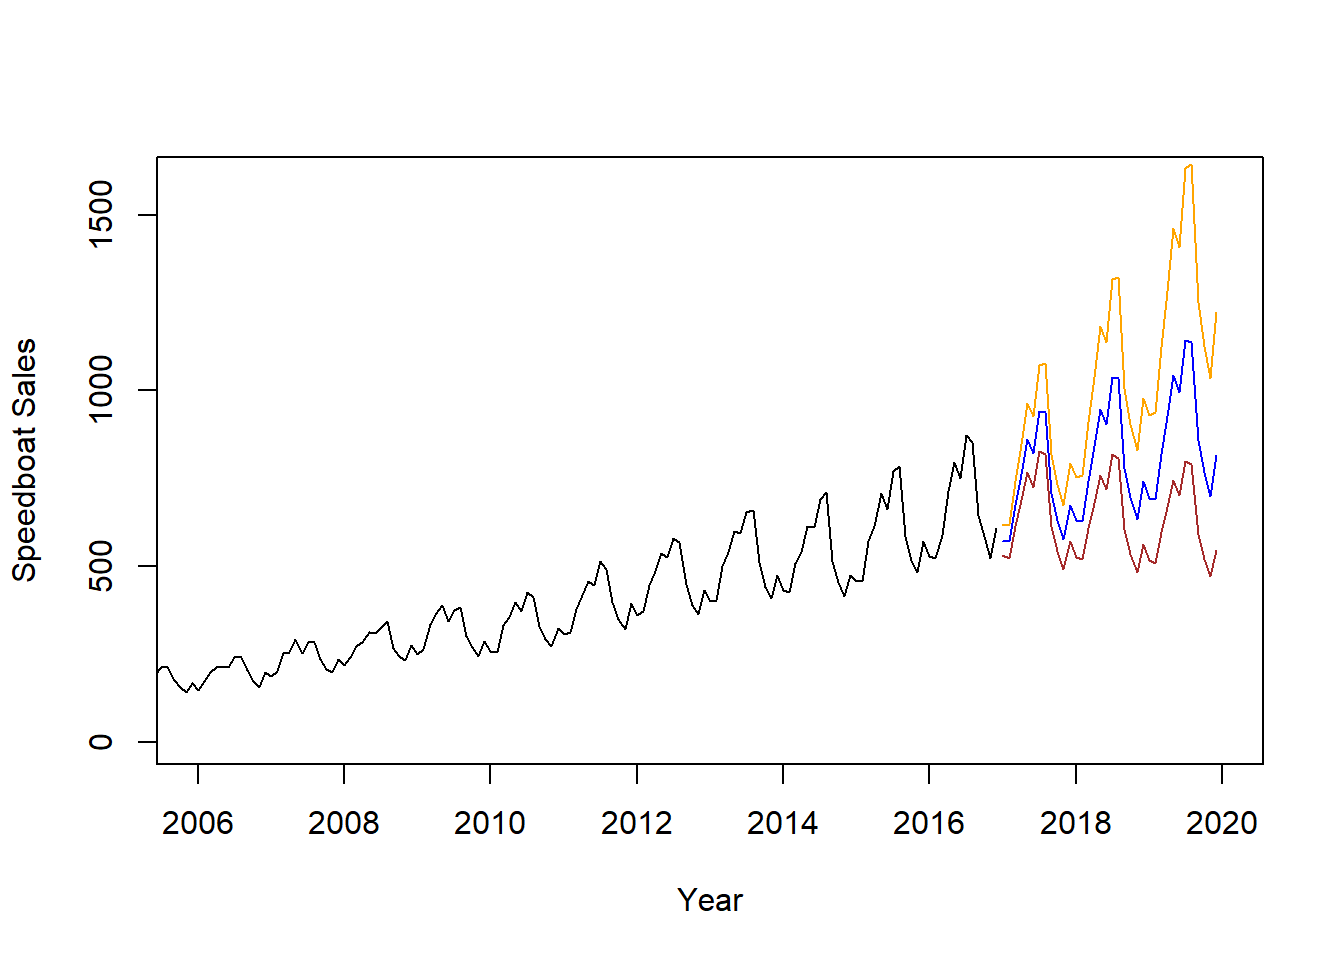
\includegraphics[]{00-B2/images/Speedboat_Sales_forecast.png}

%%%%%%%%%%%%%%%%%%%%%%%%%%%%%%%%%%%%%%%%%%%%%%%%%%%%%%%
\newpage 



\subsection*{Exercise 9}
\noindent Plot ACF and PACF plot of the residuals of the best fit ARIMA model and comment
on the results.


\begin{verbatim}
par(mfrow=c(1,2))
acf(ts(ARIMAfit$residuals),main="ACF Residual")

pacf(ts(ARIMAfit$residuals),main="PACF Residual")
\end{verbatim}

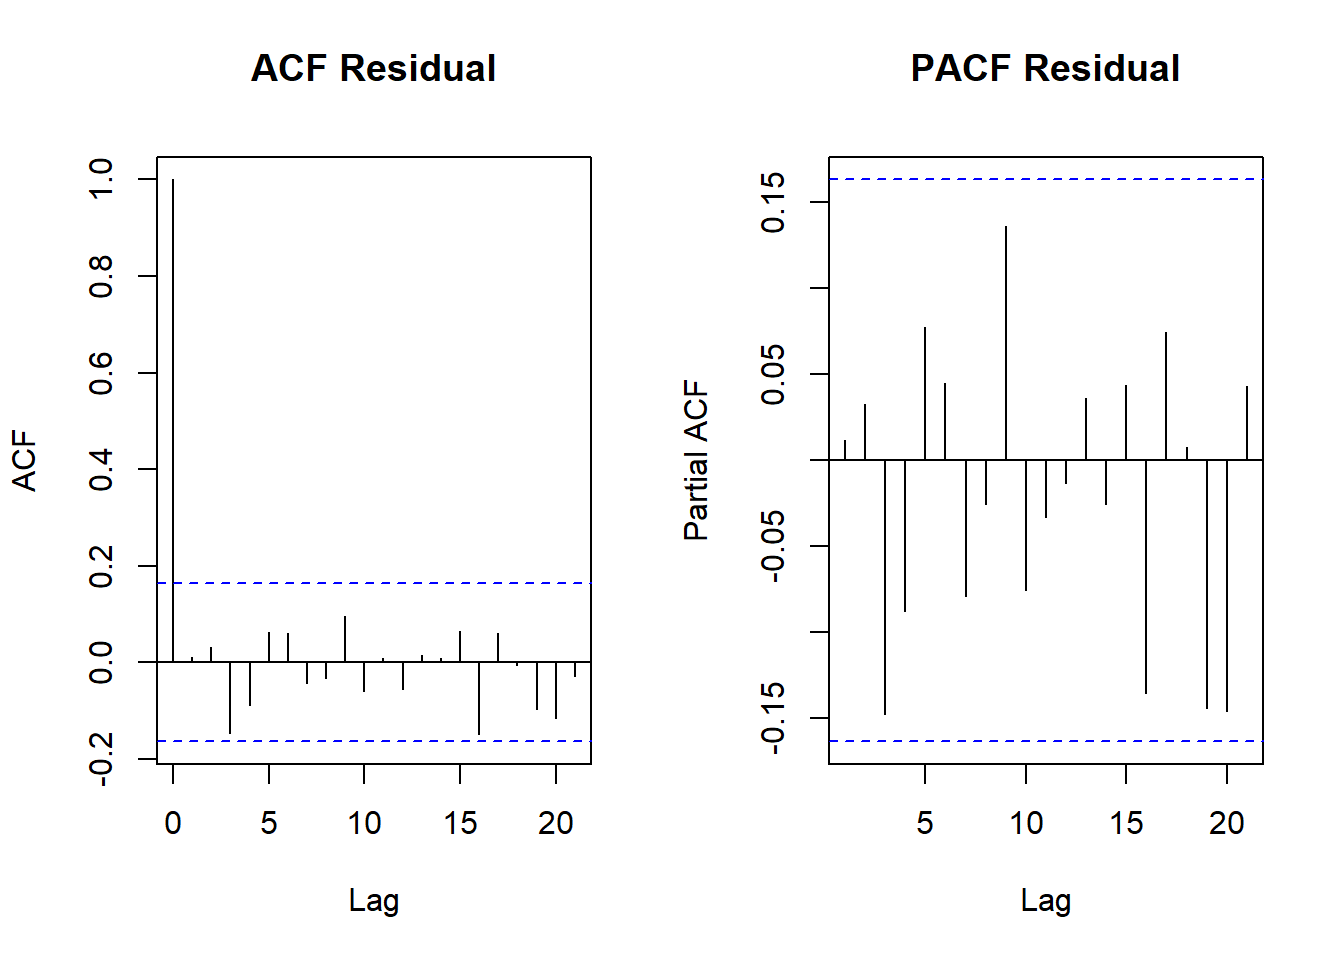
\includegraphics[]{00-B2/images/Speedboat_Sales_8.png}

\noindent Since there are no spikes outside the insignificant zone for both ACF and PACF plots we can conclude
that residuals are random with no information or juice in them. Hence our ARIMA model is working
fine.
\newpage
BLANK
\end{document}